% article.tex, a sample LaTeX file.
% Run LaTeX on this file twice for proper section numbers.
% A '%' causes LaTeX to ignore remaining text on the line

% Use the following line for draft mode (double spaced, single column)
\documentclass[preprint,pre,floats,aps,amsmath,amssymb]{revtex4}

% Use the following line for journal mode (single spaced, double
%column)
%\documentclass[twocolumn,pre,floats,aps,amsmath,amssymb]{revtex4}
\usepackage{graphicx}
\usepackage{bm}
\usepackage{hyperref}




\graphicspath{ {../data/new/images/} }


\begin{document}

\title{Replication}
\author{Gleb Pashchenko}
\affiliation{New Economic School}
\date{\today}



\maketitle




\section{Introduction}
\label{sec:intro}

In the article "Econometric measures of connectedness and systemic risk" Billio et al. \cite{billio} use a combination of econometric techniques to study the level of connectedness. They use data from 1994 to 2008 exploring the build up to the financial crisis. The main idea of their study is to find support using econometric techniques for the intuitive idea of the increase in the interconnectedness of the financial system. It is a widely shared belief that severity of the financial crisis was partially explained by  excessive interconnectedness. In presence of leverage and value-at-risk constraints shocks in the systems could be amplified by the interconnectedness. Increased volatility would require managers to "fly to quality" which would provide increased pressure on prices and start a vicious cycle. In the interconnected system a failure of couple key players can result in huge system-wide losses. 

Billio et al.  work is about measuring this interconnectedness and finding metrics that could be predictive of the heightened system-wide risk. They propose simple but novel in application metrics to measure interconnectedness, including principal components analysis, GARCH system variance, and various measures associated with pairwise Granger causality test. To calculate their metrics they split financial system into four groups: brokers, banks, insurers and hedge funds. Their conjecture  is that relations between the groups became closer in the build up to the financial crisis. It is important to note that Billio et al. limit their sample to the 25 biggest institutions in each category, since interconnectedness as a risk should be most important for them.  Therefore, the sample is dynamically updating. To determine 25 biggest institutions, they calculate the average size (market cap or AUM) for the rolling 36 months period. 



In my work I replicate their research and also extend their analysis by using longer data frame to see how their metrics behave after financial crisis and also  proposing my own metrics, including intra and inter group variation and  significance of VAR coefficients.

Throughout article I will show two pictures side by side: result from my replication on the left and result from Billio~\cite{billio} on the right. 


\section{Data}
\label{sec:data}
At first, I did not have access to data that Billio et al.  used. I used Bloomberg to download data for all types using the same SIC code as in paper. I did not limit my search to currently active funds. I faced two problems. First of all, there was no data on hedge funds and second of all observations for early dates were very scarce, for example there were only 14 broker-dealers for 1994 while I needed 25 securities for the analysis similar to Billio et al. 
\indent
I did not have data on hedge funds, so I asked my classmate who used data from CISDM Morningstar database for hedge funds returns. This is not the same database as in Billio et al. (they use Lipper Hedge Fund Database), but I had to use what I had. 

  
\indent
Later I found out that Mila Sherman actually responded to my message and shared data as well as partial MatLab code. I found this message in my spam folder and was really surprised. Data on hedge funds was missing but I recreated it using data that was shared by my classmate. 

\indent
I also extended files shared with me using my own data parsed from Bloomberg and CISDM Morningstar database, so now I had observations until Jan 2018. The shared files were in xls format with 144 sheets, where each had top 100 financial institutions and observations for 36 month rolling period. To extend data I followed the same procedure as in Billio et al., sorting by market cap at each 36 month rolling period and selecting biggest 25 in the following categories: brokers, insurers,banks and hedge funds. Replication of the summary of the data is in the appendix.






\section{Replication}
\label{sec:insample}
\subsection{GARCH}

I start with reproducing Garch (1,1) results.  For this I calculate mean of all institutions for each rolling 36 month window and apply Garch (1,1) model to predict variance of the system.

First of all, residuals do not look normal. The p-value of the null that residuals are normally distributed is very small. However, closer examination gives insight that it is mainly because of 2008 where extremely low returns skewed the results. Billio did not use log transformation that is commonly applied to financial data. I tried doing log transformation but this did not affect the results. 
The Box-Ljung test's p-value is well above zero which means that we cannot reject the null that squared residuals do not exhibit serial correlations after applying Garch. 

Thre is a clear spike in 2008 and then reduction of pressure from the standpoint of a system`s variance. Billio et al. analysis implied that this spike is related to increase of interconnectedness, however this does not seem to be the case, since the GARCH measure quickly fell on the extended data after 2008, however the interconnectedness of the system has probably remained on the same level. 



\begin{figure}[ht]
\includegraphics[width=2.8 in]{partialgarch.jpeg}
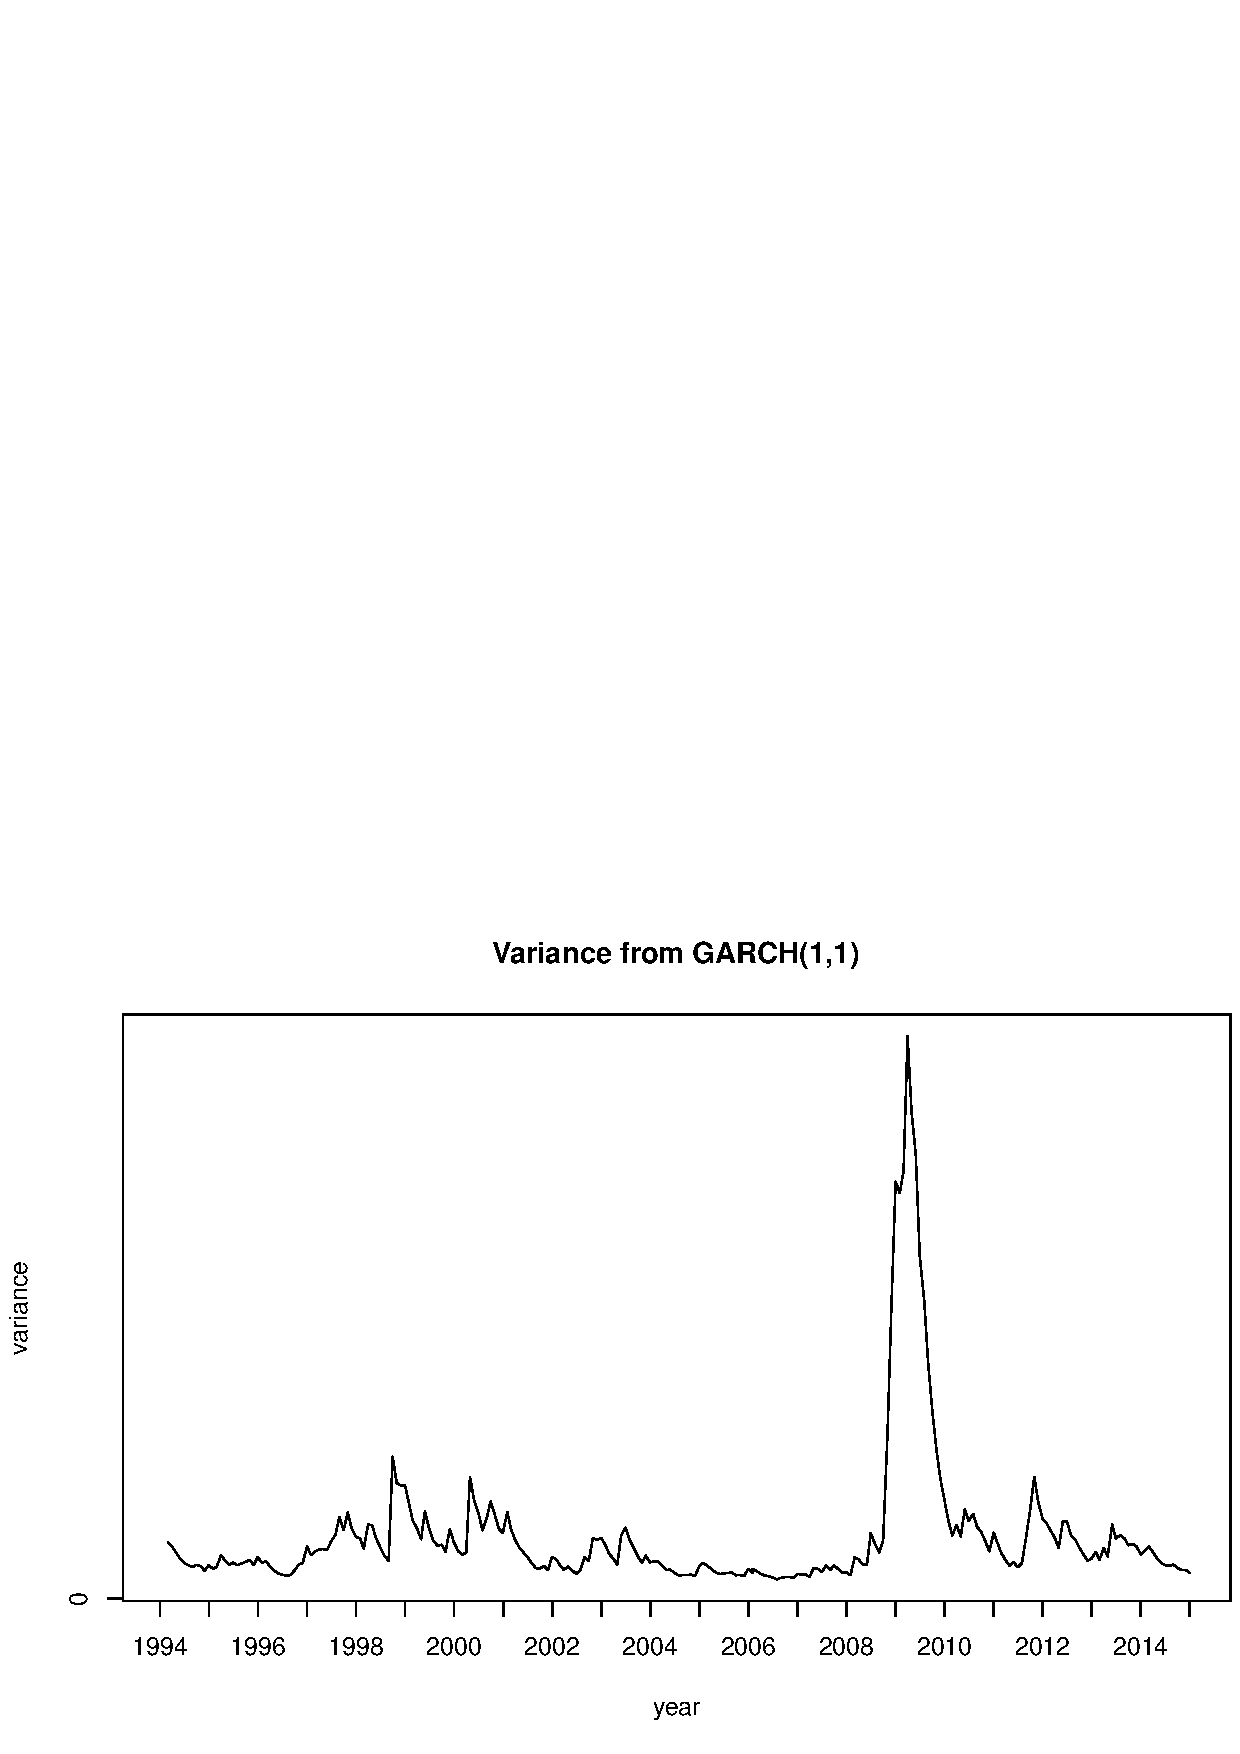
\includegraphics[width=2.8 in]{fullgarch.jpeg}
\includegraphics[width=2.8 in]{Billio Results/theirGarch.PNG}
\caption{Results from GARCH estimation for sample similar to Billio (left), for full sample(right) and from \cite{billio} (bottom) }

\end{figure}


\subsection{PCA}
I reproduce PCA results calculating variance explained by first principal components. For each 36 month rolling window I transform the data into lower dimensional space. Eigenvalues of the matrix represent variance of the data after transformation (they are matched with vectors representing principal components). Using all 36 principal components would mean that there is no loss of information in the transformed data and therefore we can calculate proportion of variance left relative to the case of 36 components. 

It is worth noting that proportion explained by the first principal component increased in the build up to the financial crisis and stayed at the sligthly elevated elevated level. I tested this relationship using CHOW test with a break before 2006 and did not find significant results.

\begin{figure}[ht]
\includegraphics[width=2.8 in]{pca_explained.jpeg}
\includegraphics[width=2.8 in]{Billio Results/PCA.PNG}

\caption{Proportion explained by principal components from PCA }

\end{figure}



\subsection{Granger Causality Graph}

Time-series $i$ Granger causes time-series $j$ if adding lags of $i$ to lags of $j$ improves forecast of $j$. Billio et. al use BIC criterion to specify number of lags included in the model. For visual illustration they show the picture of the graph where each arrow from institution $i$ to institution $j$ means that institutions $i$ Granger causes institution $j$.   The density of resulting graph serves as a proxy of interconnectedness of the system. The resulting graphs for two time periods are plotted on figures  \ref{fig:granger1} and \ref{fig:granger2}. I also calculate connections for 2018 which show that financial system is still on level of the interrelatedness of 2008 (figure  \cite{fig:granger3})

\begin{figure}[ht]
\includegraphics[width=3 in]{graph94_order_3.jpeg}
\includegraphics[width=3 in]{Billio Results/graph94.png}

\caption{Graph for 1994-1996. Mine on the left, theirs on the right }
\label{fig:granger1}
\end{figure}

\begin{figure}[ht]
\includegraphics[width=3 in]{graph_08_fin.jpeg}
\includegraphics[width=3 in]{Billio Results/graph2006.PNG}

\caption{Graph for 2006-2008. Mine on the left, theirs on the right }
\label{fig:granger2}
\end{figure}

\begin{figure}[ht]
\includegraphics[width=6 in]{2018.png}

\caption{Graph for 2018 }
\label{fig:granger3}
\end{figure}


I also calculate number of significant granger causality connections for the rolling period (figure \ref{fig:rollingGranger}). The only caveat that I only calculate points for every 6 months because of computation speed.


\begin{figure}[ht]
\includegraphics[width=3 in]{Significant Granger.png}
\includegraphics[width=3 in]{Billio Results/granger causality relationships.PNG}

\caption{Graph for 2006-2008. Mine on the left, theirs on the right }
\label{fig:rollingGranger}
\end{figure}




\section{Out of sample results}

\section{Extension}

\begin{figure}[ht]
\includegraphics[width=6 in]{change in sample.png}

\caption{Change in sample. Vertical axis represents number of institutions within top 100 that are changed each month}
\label{fig:change}
\end{figure}


It is important to note that essentially Billio et al. uses rotating sample. For each 36 rolling window selection of institutions changes and one can wonder whether some of the results could be explained by rotation of institutions. As a robustness check I looked at number of changes from one month to next (figure \ref{fig:change}). Figure could be split into two parts: pre 2008 and post 2008, Billio et al. studied only pre 2008 part and for that part plot looks homogeneous. 
 

\subsection{Pooled Analysis}

\begin{figure}[ht]
\includegraphics[width=6 in]{means.png}

\caption{Plot of aggregated means }
\label{fig:means}
\end{figure}


Let us at first step away from the granularity considered in Billio et. al. For that I computed indices for brokers, insurers, banks and hedge funds. Means for each type are graphed on figure \ref{fig:means}. Let us check whether unit root is present in these processes.  Using augmented Dickey Fueller test we find that p-value is insignificant on the 5\% level. In fact for hedge the statistic is right on the boundary and visual analysis suggests that there might be a structural break after 2005 -  returns are severely compressed on the right part of the picture. One possible explanation for that might be imperfections in the database which resulted in the survivorship bias. Nevertheless, I proceed and examine F-static for splitting regression into two parts (Figure \ref{fig:hf_break}), which shows that there might indeed be a structural break. The supremum of the F static is significant.  One of the reasons for structural break around 2006-2007 might be in the increased leverage of the financial system or interconnectedness which might have had spillover effects on the hedge funds returns. Or perhaps the whole system underwent a structural break and for hedge funds it was just quicker to notice since there is much less variability in hedge fund returns. To test for this I examine the structural breaks of the whole system and using Chow test for the VAR model find that there is indeed a structural break. 


\begin{figure}[ht]
\includegraphics[width=6 in]{structural break.png}

\caption{Structural break for hedge funds }
\label{fig:hf_break}
\end{figure}

As a variation on Billio et al. pairwise Granger causality idea I used the number of significant coefficients in the rolling VAR model for constructed indices. Results are presented in the figure \ref{fig:signVAR}. The results are  qualitatively similar to Billio et al. 

\begin{figure}[ht]
\includegraphics[width=3 in]{varsig.png}
\includegraphics[width=3 in]{Billio Results/granger causality relationships.png}

\caption{Number of significant coefficients in a rolling VAR on means of brokers, insurers, hedge funds and banks with a window of 50 months (left) and number of granger as percent of all connection from Billio (right)}
\label{fig:signVAR}
\end{figure}




\subsection{Inter and intra group variation}

A logical way to look at the interconnectedness of the system would be to look at a variation within groups and across groups. Presumably with the increase of interconnectedness variation across groups should become smaller while effect on within group variation is ambiguous. The two crisis stand out on the left and right figure. However, it should be noted that variance within the groups was higher in 2000 while variance between the groups was higher in 2008. 

\begin{figure}[ht]
\includegraphics[width=3 in]{variance within groups.png}
\includegraphics[width=3 in]{intragroup.png}

\caption{Variance within groups on the left and across groups on the right }
\end{figure}





\cleardoublepage
\appendix*

\section{Sample summary}

\begin{figure}[t]
\includegraphics[width=5 in]{Billio Results/Billio_table1_summary.png}
\caption{Summary Table from \cite{billio}}
\label{fig:billiosummary}
\end{figure}

\indent
Below is summary of data that replicates figure~\ref{fig:billiosummary}. Full sample results are different because I also added data from 2008 onwards. Billio perhaps confusingly uses annualized values for mean and median but simple monthly min and max. I calculated all statistics for annualized variables. 



\clearpage
{\centering\textbf{My Summary}\par}


% Table created by stargazer v.5.2.2 by Marek Hlavac, Harvard University. E-mail: hlavac at fas.harvard.edu
% Date and time: ��, ��� 20, 2019 - 18:55:17
\begin{table}[!htbp] \centering 
  \caption{Full sample} 
  \label{} 
\begin{tabular}{@{\extracolsep{5pt}} ccccccccccc} 
\\[-1.8ex]\hline 
\hline \\[-1.8ex] 
type & Min. & 1st Qu. & Median & Mean & 3rd Qu. & Max. & Std. Dev & Skew & kurtosis & autocorrelation \\ 
\hline \\[-1.8ex] 
banks & $$-$9.70$ & $$-$0.42$ & $0.16$ & $0.13$ & $0.70$ & $25$ & $1.36$ & $2.99$ & $56.72$ & $$-$0.02$ \\ 
brokers & $$-$10$ & $$-$0.54$ & $0.17$ & $0.18$ & $0.82$ & $35$ & $1.47$ & $1.92$ & $22.51$ & $0$ \\ 
hedge funds & $$-$7.70$ & $$-$0.05$ & $0.09$ & $0.09$ & $0.22$ & $5.70$ & $0.40$ & $0.46$ & $25.58$ & $0.14$ \\ 
insurers & $$-$10$ & $$-$0.38$ & $0.15$ & $0.15$ & $0.65$ & $20$ & $1.28$ & $2.61$ & $45.88$ & $$-$0.05$ \\ 
\hline \\[-1.8ex] 
\end{tabular} 
\end{table} 


% Table created by stargazer v.5.2.2 by Marek Hlavac, Harvard University. E-mail: hlavac at fas.harvard.edu
% Date and time: ��, ��� 20, 2019 - 18:55:18
\begin{table}[!htbp] \centering 
  \caption{January 1994-December 1996} 
  \label{} 
\begin{tabular}{@{\extracolsep{5pt}} ccccccccccc} 
\\[-1.8ex]\hline 
\hline \\[-1.8ex] 
type & Min. & 1st Qu. & Median & Mean & 3rd Qu. & Max. & Std. Dev & Skew & kurtosis & autocorrelation \\ 
\hline \\[-1.8ex] 
banks & $$-$2.30$ & $$-$0.23$ & $0.27$ & $0.29$ & $0.80$ & $5.30$ & $0.82$ & $0.31$ & $1.87$ & $0.01$ \\ 
brokers & $$-$4.20$ & $$-$0.40$ & $0.18$ & $0.23$ & $0.82$ & $5.60$ & $1.01$ & $0.25$ & $1.46$ & $$-$0.07$ \\ 
hedge funds & $$-$2.10$ & $$-$0.04$ & $0.11$ & $0.12$ & $0.25$ & $3.20$ & $0.42$ & $0.99$ & $10.12$ & $0.21$ \\ 
insurers & $$-$3.10$ & $$-$0.27$ & $0.16$ & $0.20$ & $0.67$ & $5.80$ & $0.82$ & $0.66$ & $3.91$ & $$-$0.09$ \\ 
\hline \\[-1.8ex] 
\end{tabular} 
\end{table} 


% Table created by stargazer v.5.2.2 by Marek Hlavac, Harvard University. E-mail: hlavac at fas.harvard.edu
% Date and time: ��, ��� 20, 2019 - 18:55:19
\begin{table}[!htbp] \centering 
  \caption{January 1996-December 1998} 
  \label{} 
\begin{tabular}{@{\extracolsep{5pt}} ccccccccccc} 
\\[-1.8ex]\hline 
\hline \\[-1.8ex] 
type & Min. & 1st Qu. & Median & Mean & 3rd Qu. & Max. & Std. Dev & Skew & kurtosis & autocorrelation \\ 
\hline \\[-1.8ex] 
banks & $$-$4.40$ & $$-$0.20$ & $0.35$ & $0.34$ & $0.91$ & $5.60$ & $1.04$ & $$-$0.18$ & $2.83$ & $$-$0.09$ \\ 
brokers & $$-$10$ & $$-$0.42$ & $0.24$ & $0.31$ & $1.10$ & $20$ & $1.67$ & $2.87$ & $40.02$ & $0.01$ \\ 
hedge funds & $$-$3.20$ & $0.004$ & $0.12$ & $0.13$ & $0.28$ & $3.30$ & $0.50$ & $0.43$ & $9.78$ & $0.10$ \\ 
insurers & $$-$7.90$ & $$-$0.35$ & $0.24$ & $0.24$ & $0.86$ & $8.30$ & $1.08$ & $$-$0.23$ & $8.86$ & $$-$0.01$ \\ 
\hline \\[-1.8ex] 
\end{tabular} 
\end{table} 


% Table created by stargazer v.5.2.2 by Marek Hlavac, Harvard University. E-mail: hlavac at fas.harvard.edu
% Date and time: ��, ��� 20, 2019 - 18:55:20
\begin{table}[!htbp] \centering 
  \caption{January 1999-December 2001} 
  \label{} 
\begin{tabular}{@{\extracolsep{5pt}} ccccccccccc} 
\\[-1.8ex]\hline 
\hline \\[-1.8ex] 
type & Min. & 1st Qu. & Median & Mean & 3rd Qu. & Max. & Std. Dev & Skew & kurtosis & autocorrelation \\ 
\hline \\[-1.8ex] 
banks & $$-$6.10$ & $$-$0.61$ & $0.06$ & $0.13$ & $0.83$ & $5.90$ & $1.21$ & $0.27$ & $2.24$ & $$-$0.06$ \\ 
brokers & $$-$5.50$ & $$-$0.93$ & $0.08$ & $0.28$ & $1.20$ & $19$ & $2.42$ & $2.18$ & $11.49$ & $$-$0.01$ \\ 
hedge funds & $$-$2.80$ & $0.002$ & $0.10$ & $0.12$ & $0.26$ & $3.50$ & $0.53$ & $0.80$ & $8.37$ & $0.16$ \\ 
insurers & $$-$7.10$ & $$-$0.77$ & $0.01$ & $0.10$ & $0.75$ & $10$ & $1.46$ & $0.82$ & $5.05$ & $$-$0.14$ \\ 
\hline \\[-1.8ex] 
\end{tabular} 
\end{table} 


% Table created by stargazer v.5.2.2 by Marek Hlavac, Harvard University. E-mail: hlavac at fas.harvard.edu
% Date and time: ��, ��� 20, 2019 - 18:55:20
\begin{table}[!htbp] \centering 
  \caption{January 2002-December 2004} 
  \label{} 
\begin{tabular}{@{\extracolsep{5pt}} ccccccccccc} 
\\[-1.8ex]\hline 
\hline \\[-1.8ex] 
type & Min. & 1st Qu. & Median & Mean & 3rd Qu. & Max. & Std. Dev & Skew & kurtosis & autocorrelation \\ 
\hline \\[-1.8ex] 
banks & $$-$3.20$ & $$-$0.30$ & $0.17$ & $0.14$ & $0.60$ & $3.60$ & $0.78$ & $$-$0.15$ & $1.26$ & $$-$0.09$ \\ 
brokers & $$-$3.30$ & $$-$0.62$ & $0.14$ & $0.10$ & $0.77$ & $4.90$ & $1.14$ & $0.11$ & $1.04$ & $0.04$ \\ 
hedge funds & $$-$1.60$ & $0.004$ & $0.07$ & $0.09$ & $0.16$ & $2$ & $0.26$ & $0.87$ & $12.06$ & $0.21$ \\ 
insurers & $$-$5.90$ & $$-$0.35$ & $0.12$ & $0.12$ & $0.61$ & $3.30$ & $0.87$ & $$-$0.52$ & $4.16$ & $0.03$ \\ 
\hline \\[-1.8ex] 
\end{tabular} 
\end{table} 


% Table created by stargazer v.5.2.2 by Marek Hlavac, Harvard University. E-mail: hlavac at fas.harvard.edu
% Date and time: ��, ��� 20, 2019 - 18:55:21
\begin{table}[!htbp] \centering 
  \caption{January 2006-December 2008} 
  \label{} 
\begin{tabular}{@{\extracolsep{5pt}} ccccccccccc} 
\\[-1.8ex]\hline 
\hline \\[-1.8ex] 
type & Min. & 1st Qu. & Median & Mean & 3rd Qu. & Max. & Std. Dev & Skew & kurtosis & autocorrelation \\ 
\hline \\[-1.8ex] 
banks & $$-$9.40$ & $$-$0.68$ & $$-$0.07$ & $$-$0.24$ & $0.41$ & $10$ & $1.40$ & $$-$1.05$ & $10.19$ & $0.07$ \\ 
brokers & $$-$9$ & $$-$0.71$ & $0.09$ & $$-$0.05$ & $0.72$ & $14$ & $1.48$ & $0.25$ & $12.96$ & $0.17$ \\ 
hedge funds & $$-$2.50$ & $$-$0.13$ & $0.07$ & $0.03$ & $0.22$ & $3.20$ & $0.42$ & $$-$0.44$ & $7.62$ & $0.25$ \\ 
insurers & $$-$10$ & $$-$0.51$ & $0.02$ & $$-$0.15$ & $0.46$ & $11$ & $1.46$ & $$-$0.58$ & $17.09$ & $0.12$ \\ 
\hline \\[-1.8ex] 
\end{tabular} 
\end{table} 

\clearpage
\par

\section{Notes}
\subsection{Data}
I used EQS function in Bloomberg to screen for securities. File "returns.xlsx" has all the tickers from Bloomberg with market capitalizations at 7 different points at time. For speed, I used Python to filter top 25 for each period in time (file "clean.ipynb"). At the end I produced file "picks.xlsx" which summarizes whether given ticker was included in the top 25 for a given period. I also saved into "backup" folder csv files with top 25 in each category across the time (by using number of non-null observations as sorting mechanism and average market cap if number of tickers with non-null observations is higher than 25). 
\indent
All data cleaning related to hedge funds is in folder "hedge fund" . I was given files "active\textunderscore info.csv", "active\textunderscore returns.csv", "dead funds\textunderscore info.csv", "dead funds\textunderscore returns.csv". I selected hedge funds conditioning on having at least 140 returns in a 180 month period and maximum average NAV (file "selection.csv") and "hedge funds.csv".

\indent
Files that were shared by Sherman are in the folder "FilesFromSherman". To recreate hedge fund data I used Python for speed, (Python file is hedge fund/newattempt/hedge fund data.ipynb, output file is in hedge fund/newattempt/hf\textunderscore result.xlsx). The output files of data extension are in "shared/new". Code to produce this was is in "hedge fund/new attempt/get\textunderscore new\textunderscore data.ipynb". Code is not organized well because I somehow lost all my code and had to reconstruct it using R Studio`s call history. 





\begin{thebibliography}{99}

\bibitem{billio} Billio, Getmansky, Lo and Pelizzon, Journal of Financial Economics, 104 (2012)

\end{thebibliography}

\end{document}             % End of document.

